\vspace{0.5cm}


\section*{Problema 14.1}
\begin{enumerate}[a)]
	\item Encontramos $E_{x0}$, se tiene
		$$ E_{x0} = -\pdv{\varphi}{x} = \boxed{ kA\sin{kx} e^{kz}, } $$
		lo que deja claro que para el vacío se cumple la condición de frontera.
	\item Sabiendo que $D_i = \varepsilon (\omega) E_i$, se tiene que $D = \varepsilon (\omega) kA \cos{kx}$ (dado que se da a $z = 0$). Teniendo la condicion de frontera es $-kA\cos{kx}$, lo que implica que $\varepsilon (\omega) = -1$; lo que nos da $\omega _s ^2 = \frac{1}{2} \omega _p ^2$.
\end{enumerate}
	
\section*{Problema 15.5}
Partiendo de la relación dada en la ecuación $15.11a$ reemplazando, se llega a que
	$$ \varepsilon '(\omega) - 1 = \frac{4\pi ne^2}{m} P \int _0 ^\infty \frac{\delta (s - \omega _g)}{s^2 - \omega ^2} \dd{s},  $$
integrando
	$$ \varepsilon '(\omega) = \boxed{ 1 + \frac{\omega _p ^2}{\omega _g ^2 - \omega ^2}, \quad \omega _p ^2 = \frac{4\pi ne^2}{m}. } $$


\section*{Problema 17.3}
Por regla de la cadena, se tiene
	$$ D(\varepsilon) = \dv{N}{k} \dv{k}{\varepsilon} = \frac{2L^2}{4\pi ^2} *2\pi k \frac{m}{h^2 \pi} = \boxed{ \frac{mL^2}{\pi h^2}. } $$



%\section*{Anexo}
%\begin{figure}[H]
%	\centering
%	 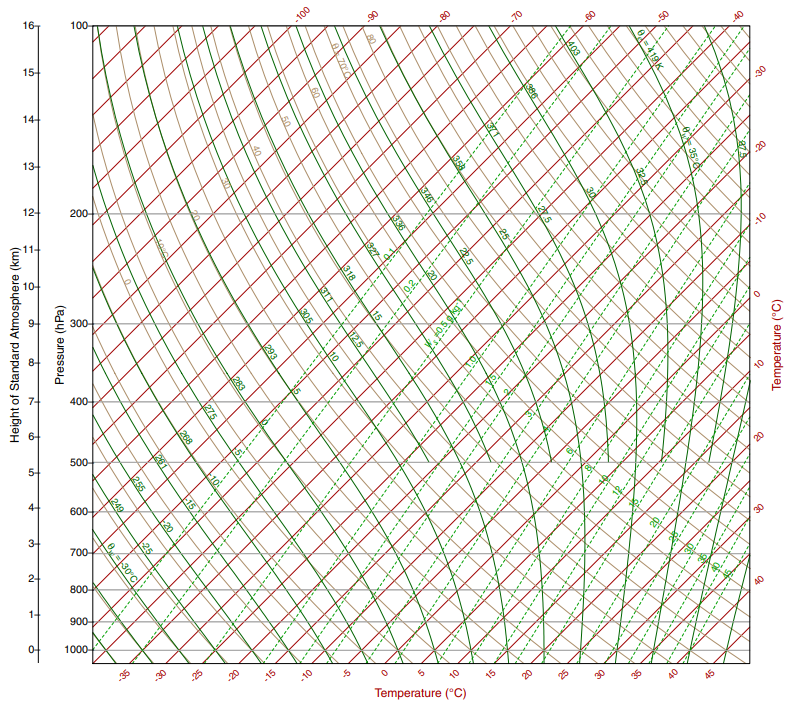
\includegraphics[scale=0.7]{./img/skewTlnp.png}
%	 \caption{Skew $T-\ln{p}$ Chart, book website.}
%	 \label{skew}
%\end{figure}



















%%%%%